\chapter{Habilidades.}
%=============================================================
	\section{Cuchillas de obsidiana} \label{hab.CuchObs}	
		\subsection{Descripción}
		El enemigo recubre su espalda con picos de obsidiana que disminuyen la cantidad de vida del jugador al hacer contacto con éste.
		\subsection{Portador}
		Armadillo (ver apartado \ref{per:armadillo})
		\subsection{Esquema}

%============================================================
		\section{Nombre: Disparo rojo.} \label{hab.disparoR}
		\subsubsection{Descripción}
El enemigo dispara tonalli de color rojo. El disparo de tonalli sale de enfrente del enemigo. El disparo de tonalli tendrá un desplazamiento horizontal constante. El disparo, al hacer contacto con el jugador, reducirá la cantidad de vida del jugador. Si el disparo colisiona con cualquier objeto, enemigo, ítem u obstáculo que no sea el jugador, el disparo se destruirá sin afectar el objeto, enemigo, ítem u obstáculo con el que haya colisionado. El disparo se destruirá si después de un periodo de tiempo no ha colisionado con ningún objeto o con el jugador.
		\subsubsection{Portador}
		Fantasma rojo. Ver \ref{per.fantasmaR}.
		\subsubsection{Esquema}
		Ver figura \ref{fig:disparoR}.
		\begin{figure}
			\centering
			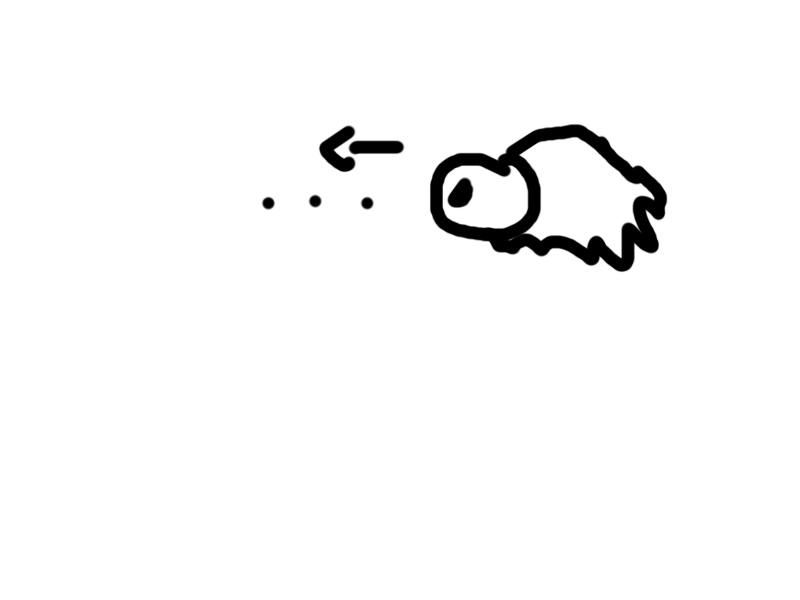
\includegraphics[height=0.2 \textheight]{Imagenes/disparoR}
			\caption{Disparo rojo.}
			\label{fig:disparoR}
		\end{figure}
			%============================================================
	\section{Nombre: Embestida.} \label{hab.embestida}
		\subsection{Descripción}
		El enemigo se desplaza en una diagonal descendente a gran velocidad.
		\subsection{Portador}
		Fantasma morado. Ver \ref{per.fantasmaM}.
		\subsection{Esquema}
		Ver figura \ref{fig:embestida}.
		\begin{figure}
			\centering
			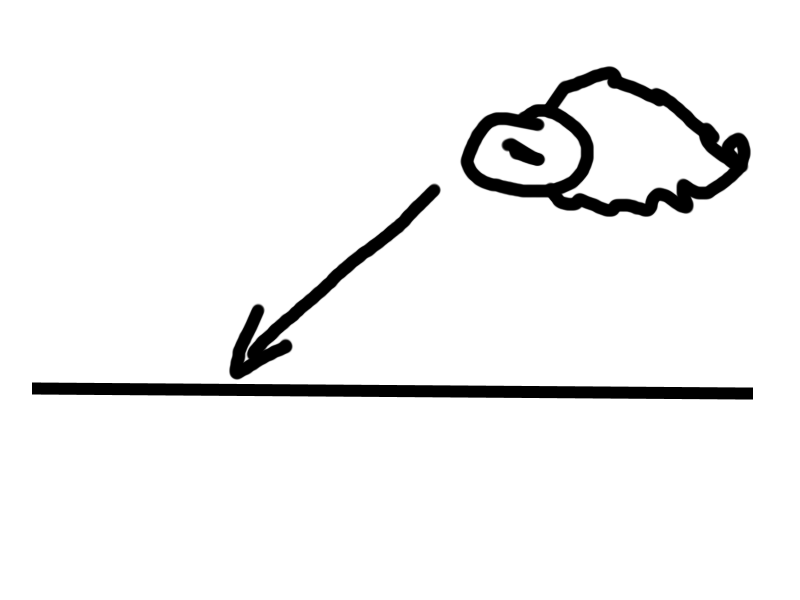
\includegraphics[height=0.2 \textheight]{Imagenes/embestida}
			\caption{Embestida.}
			\label{fig:embestida}
		\end{figure}

%============================================================
			\section{Nombre: Salto de altura.} \label{hab.SalAl}
			\subsection{Descripción}
			El enemigo describe un desplazamiento convexo de gran velocidad. 
			\subsection{Portador}
			Jaguar. Ver \ref{per.jaguar}.
			\subsection{Esquema}
			Ver figura \ref{fig:SalAl}.
			\begin{figure}
				\centering
				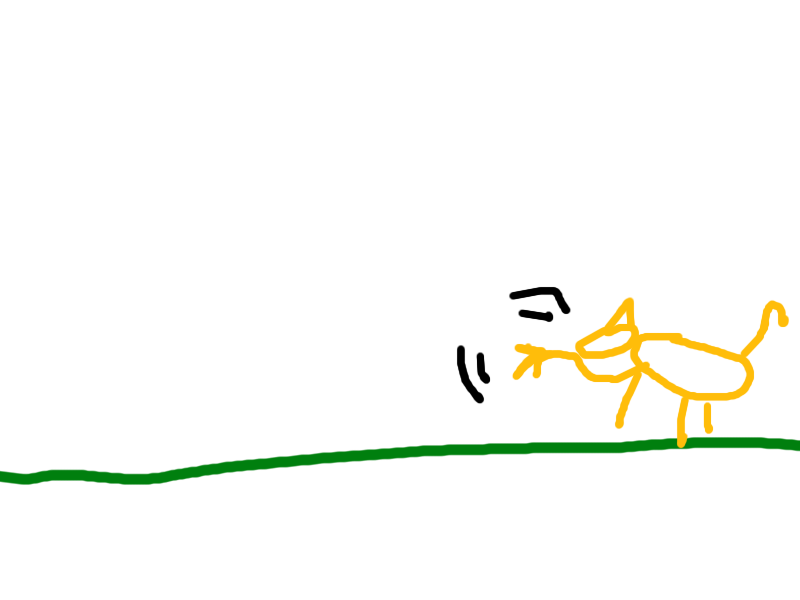
\includegraphics[height=0.2 \textheight]{Imagenes/zarpazo}
				\caption{Salto de altura.}
				\label{fig:SalAl}
			\end{figure}
			
%============================================================
\section{Nombre: Disparo de tonalli.}\label{hab.disparoT}
\subsection{Descripción}
Con ayuda de la caracola permite a su portador disparar tonalli. El disparo, al hacer contacto con el enemigo, reducirá la cantidad de vida de éste en caso de ser un jefe o lo destruirá en caso de ser un enemigo normal. Si el disparo colisiona con cualquier objeto, enemigo, ítem u obstáculo que no sea el jugador, el disparo se destruirá sin afectar el objeto, enemigo, ítem u obstáculo con el que haya colisionado. El disparo se destruirá si después de un periodo de tiempo no ha colisionado con ningún objeto u enemigo.
\subsection{Portador}
Malinalli
\subsection{Esquema}
			Ver figura \ref{fig:disparoT}.
			\begin{figure}
				\centering
				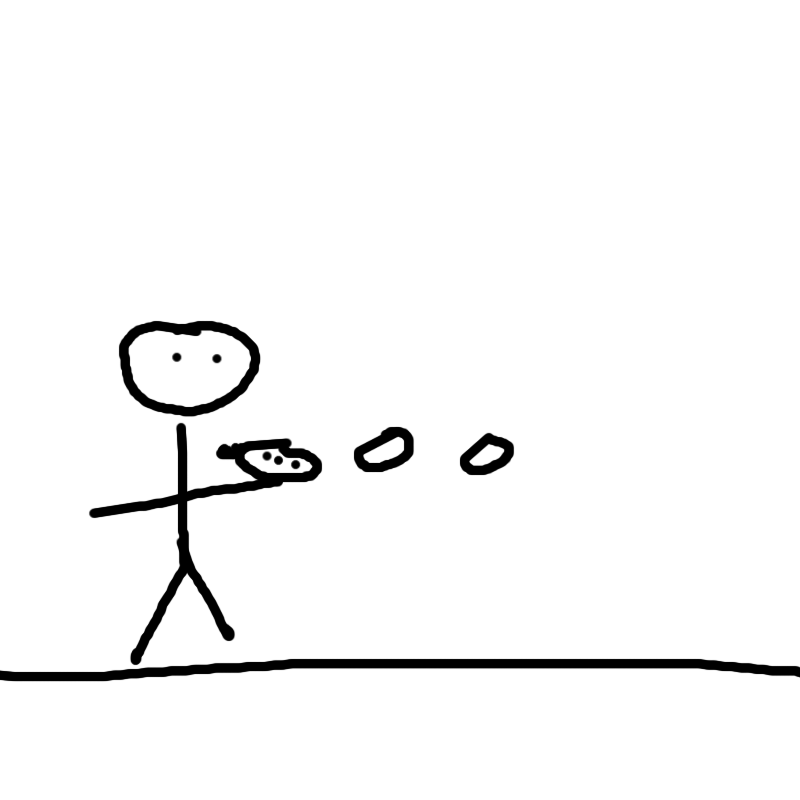
\includegraphics[height=0.2 \textheight]{Imagenes/disparoT}
				\caption{Disparo de tonalli por el jugador.}
				\label{fig:disparoT}
			\end{figure}
			
%============================================================
\section{Nombre: Zambullida.}\label{hab.zambullida}
\subsection{Descripción}
El enemigo se sumerge en el río, dejando a la vista su espalda, Una vez sumergido, el enemigo se desplaza del punto A al punto B a gran velocidad. La espalda del enemigo redice la cantidad de vida del jugador al hacer contacto con él.  
\subsection{Portador}
Zochitónal (ver apartado \ref{per:zochitonal}).
\subsection{Esquema}
			Ver figura \ref{fig:zambullida}.
			\begin{figure}
				\centering
				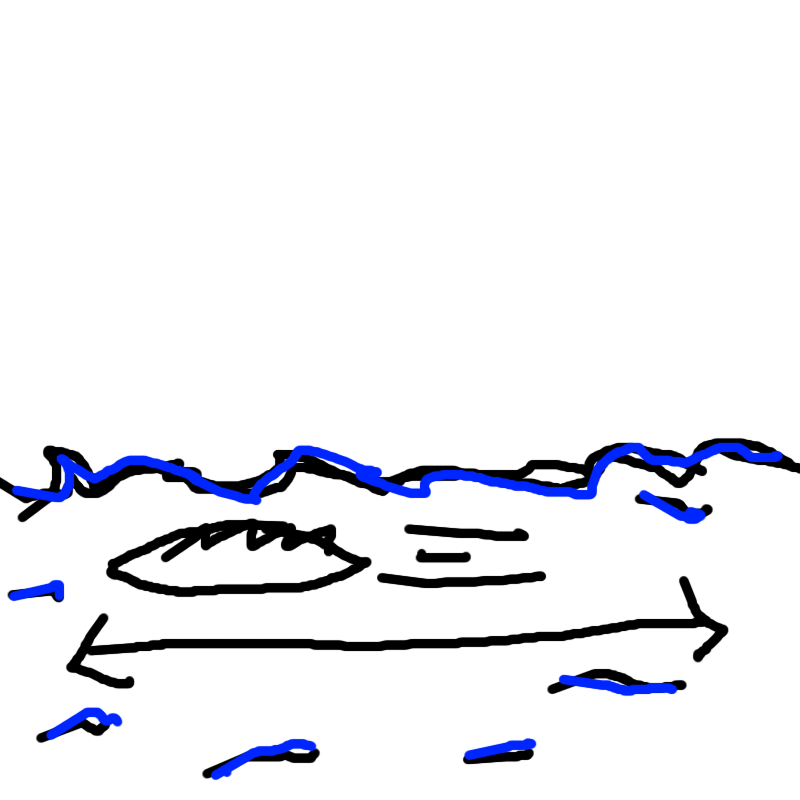
\includegraphics[height=0.2 \textheight]{Imagenes/zambullida}
				\caption{Zambullida.}
				\label{fig:zambullida}
			\end{figure}
%============================================================
\section{Nombre: Burbujas.}\label{hab.burbujas}
\subsection{Descripción}
El enemigo dispará cuatro burbujas. La burbujas seguirán al jugador durante un periodo de tiempo determinado. Cada burbuja reduce la barra de vida del jugador de manera individual al hacer colisión con el jugador. Las burbujas se destruyen al hacer contacto con el jugador, al colisionar con cualquier otro objeto o después de un tiempo si no han colisionado con ningún objeto o con el jugador. Las burbujas solo afectaran al jugador al hacer contacto con el, si colisionan con otro objeto no afectarán a ese objeto. 
\subsection{Portador}
Zochitónal (ver apartado \ref{per:zochitonal}),  Mictlantecutli (ver apartado \ref{per:mictlantecutli}).
\subsection{Esquema}
			Ver figura \ref{fig:burbujas}.
			\begin{figure}
				\centering
				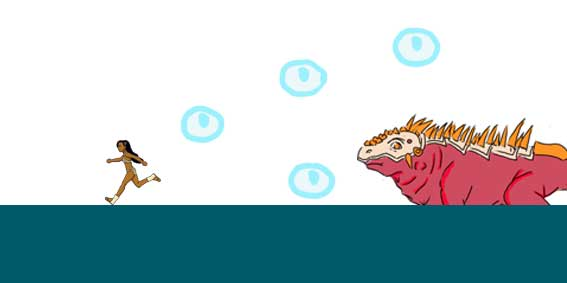
\includegraphics[height=0.2 \textheight]{Imagenes/burbujas}
				\caption{Burbujas.}
				\label{fig:burbujas}
			\end{figure}

%============================================================
\section{Nombre: Coraza.}\label{hab.coraza}
\subsection{Descripción}
Esta habilidad permite crear una coraza de piedra protegiendo a su portador de ataques enemigos sacrificando velocidad de movimiento.  
\subsection{Portador}
Tepeyóllotl (ver apartado \ref{per:tepeyollotl}).
\subsection{Esquema}
			Ver figura \ref{fig:coraza}.
			\begin{figure}
				\centering
				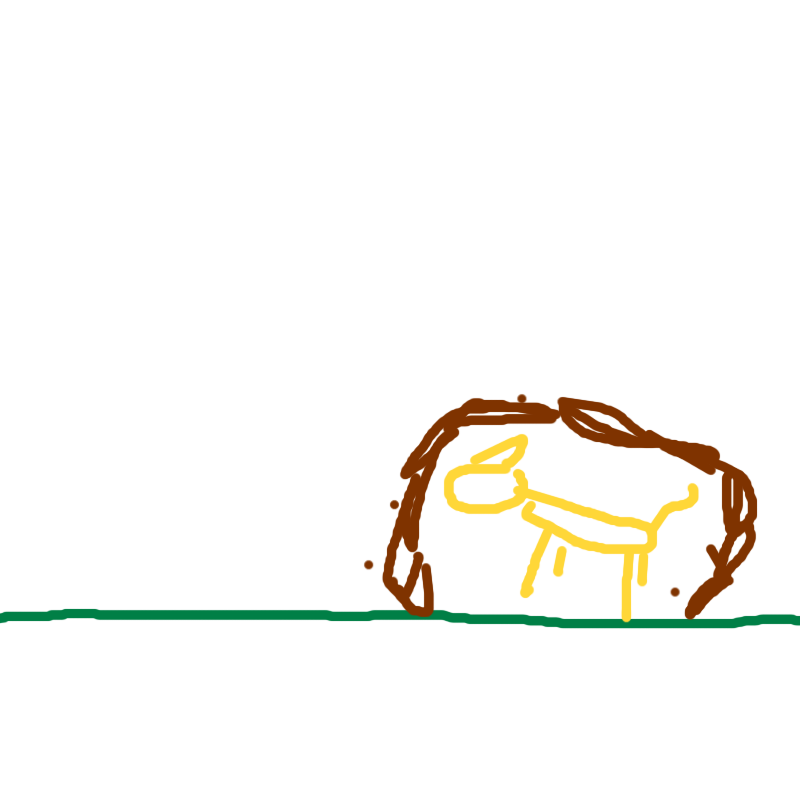
\includegraphics[height=0.2 \textheight]{Imagenes/coraza}
				\caption{Coraza.}
				\label{fig:coraza}
			\end{figure}
%============================================================
\section{Nombre: Impacto.} \label{hab.impacto}
\subsection{Descripción}
Realiza un salto, provocando al aterrizaje una onda de piedras en el suelo. El avance de las piedras se hará de manera horizontal. Las piedras infringirán disminuirán la barra de vida del jugador al hacer contacto con el. Después de un tiempo las piedras desaparecerán.
\subsection{Portador}
Tepeyóllotl (ver apartado \ref{per:tepeyollotl}).
\subsection{Esquema}

%============================================================
\section{Nombre de la habilidad: Luvia de rocas.} \label{hab.LLuviaRocas}
\subsection{Descripción}
Con un poderoso rugido se provoca una lluvia de rocas. Las rocas se destruyen al colisionar con el suelo, con una plataforma o con el jugador. Cuando las rocas colisionan con el jugador disminuyen la cantidad de la barra de vida del jugador. Las rocas no pueden destruir las plataformas o el suelo al colisionar contra estas.
\subsection{Portador}
Tepeyóllotl (ver apartado \ref{per:tepeyollotl}), Mictlantecutli (ver apartado \ref{per:mictlantecutli})..
\subsection{Esquema}
			Ver figura \ref{fig:lluviaR}.
			\begin{figure}
				\centering
				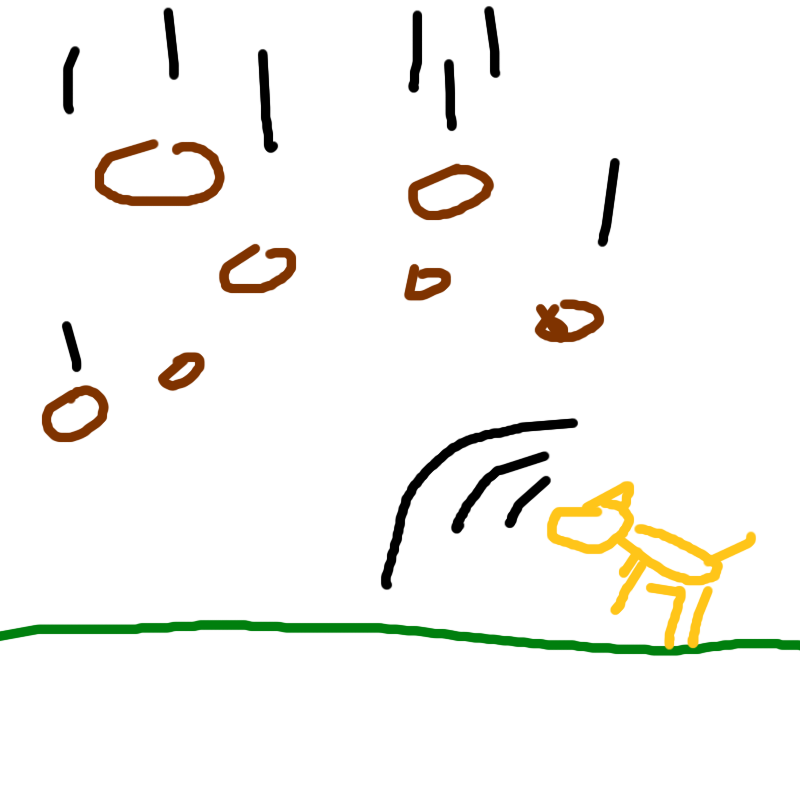
\includegraphics[height=0.2 \textheight]{Imagenes/lluviaR}
				\caption{Lluvia de rocas.}
				\label{fig:lluviaR}
			\end{figure}
			
%============================================================
\section{Nombre: Rugido aturdidor.}\label{hab.RugAtur}
\subsection{Descripción}
Poderoso rugido provoca una onda amarilla que inmoviliza a al jugador por un periodo de tiempo determinado al hacer contacto con él. La onda incrementara su diámetro hasta alcanzar un diámetro máximo, una vez alcanzado ese diámetro máximo desaparecerá. Esta habilidad solo podrá ser utilizada si su portador no tiene activa la hablidad coraza (ver apartado \ref{hab.coraza}).
\subsection{Portador}
Tepeyóllotl (ver apartado \ref{per:tepeyollotl}). 
\subsection{Esquema}
			Ver figura \ref{fig:rugido}.
			\begin{figure}
				\centering
				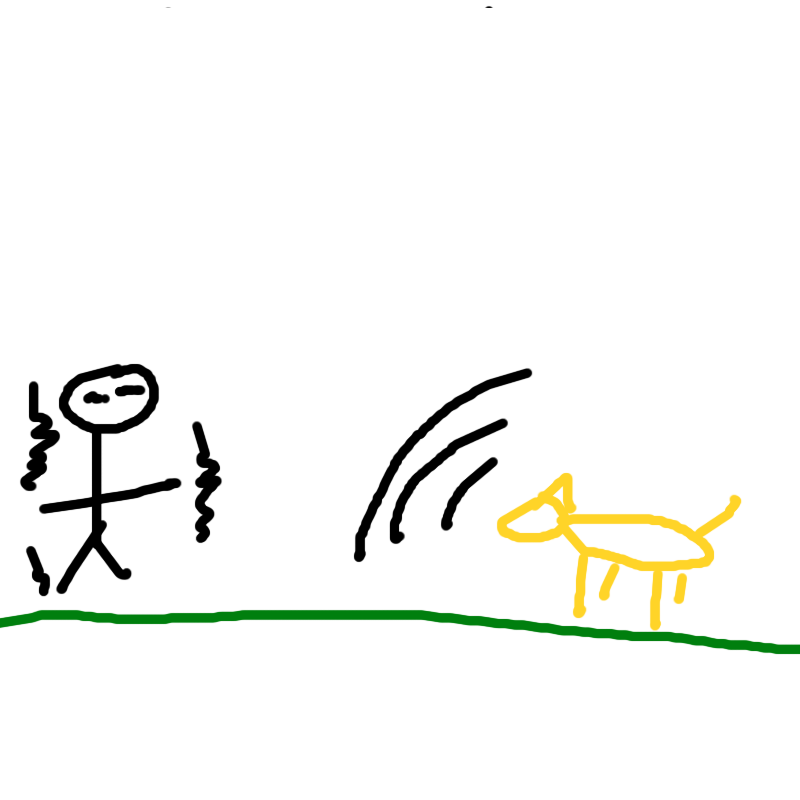
\includegraphics[height=0.2 \textheight]{Imagenes/rugido}
				\caption{Rugido aturdidor.}
				\label{fig:rugido}
			\end{figure}
			
%============================================================
\section{Nombre: Circulo de fuego.} \label{hab.CirFue}
\subsection{Descripción}
El enemigo se rodea a sí mismo con fuego, este ataque sera usado cuando el jugador se encuentre a una distancia corta del enemigo. El fuego que rodea al enemigo durara un periodo de tiempo determinado y después desaparecerá. El fuego reducirá la cantidad de vida del jugador al hacer contacto con éste. El fuego no afectara a otros objetos que no sean el jugador. Mientras esta habilidad se encuentre activa, el enemigo no recibirá daño por parte del jugador.
\subsection{Portador}
Itzpápalotl (ver apartado \ref{per:itzpapalotl}),  Mictlantecutli (ver apartado \ref{per:mictlantecutli}). 
\subsection{Esquema}
			Ver figura \ref{fig:circuloF}.
			\begin{figure}
				\centering
				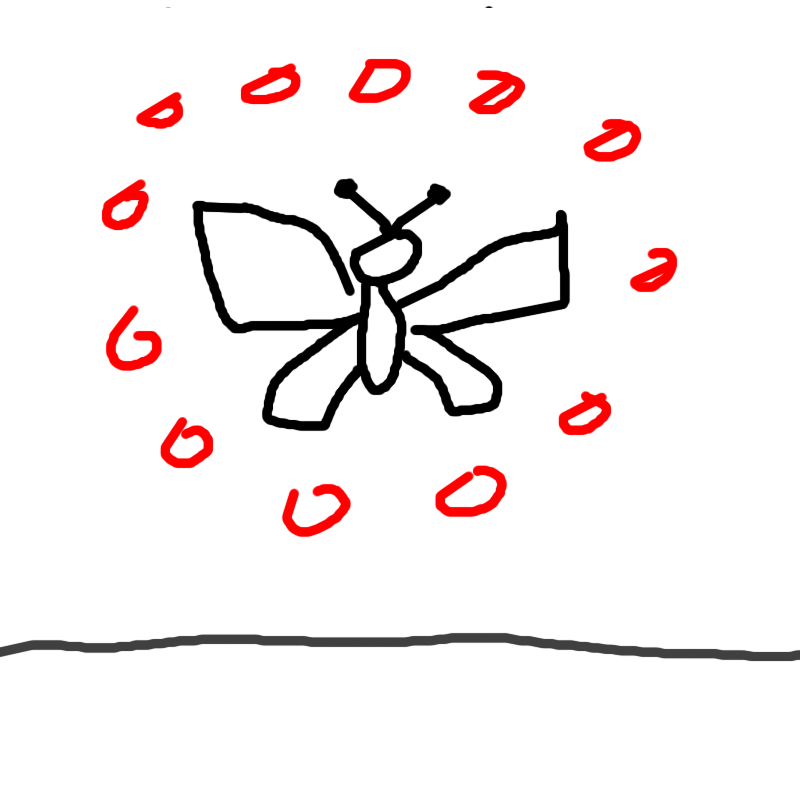
\includegraphics[height=0.2 \textheight]{Imagenes/circuloF}
				\caption{Círculo de fuego.}
				\label{fig:circuloF}
			\end{figure}
			
%============================================================
\section{Nombre: Embestida aerea.}\label{hab.EmbesAer}
\subsection{Descripción}
El enemigo usara este ataque cuando este lejos del jugador. El enemigo arremeterá a gran velocidad contra el jugador siguiendo una trayectoria de diagonal descendente.
\subsection{Portador}
Itzpápalotl (ver apartado \ref{per:itzpapalotl}).
\subsection{Esquema}
			Ver figura \ref{fig:embestidaA}.
			\begin{figure}
				\centering
				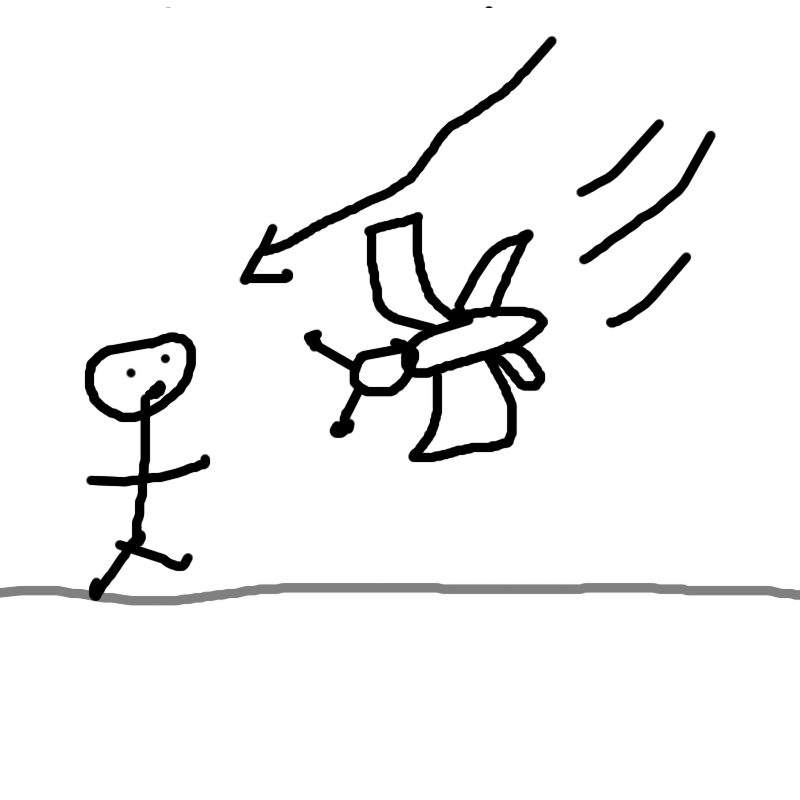
\includegraphics[height=0.2 \textheight]{Imagenes/embestidaA}
				\caption{Embestida aerea.}
				\label{fig:embestidaA}
			\end{figure}
%============================================================
\section{Nombre: Invisibilidad.} \label{hab.Invis}
\subsection{Descripción}
Esta habilidad le permite al enemigo ser indetectable al ojo de dioses y humanos, permitiendole tomar una posición ventajosa en combate.
\subsection{Portador}
Itzpápalotl (ver apartado \ref{per:itzpapalotl}).
\subsection{Esquema}
			Ver figura \ref{fig:invisibilidad}.
			\begin{figure}
				\centering
				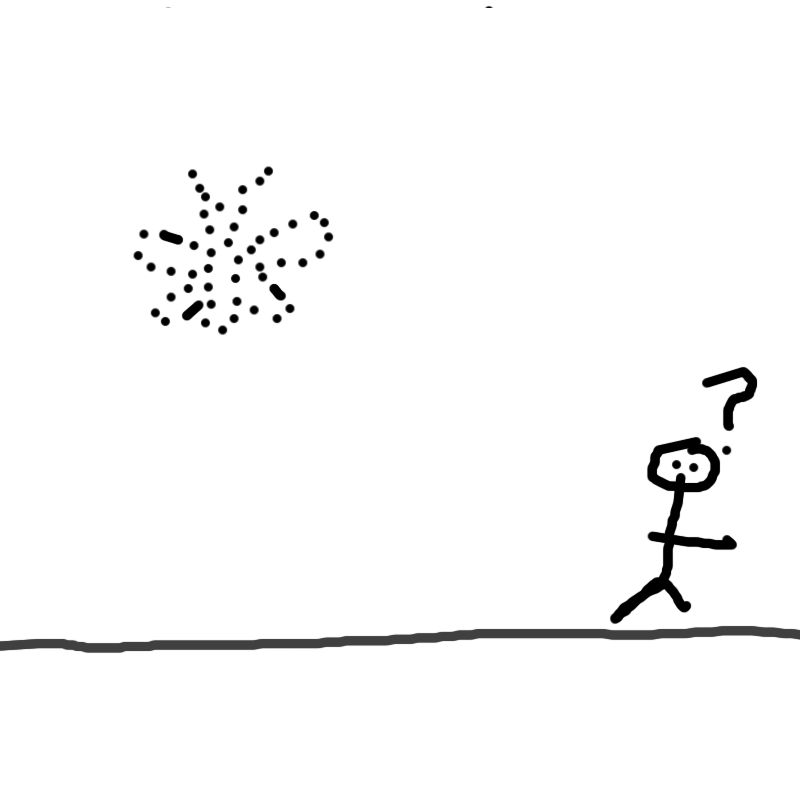
\includegraphics[height=0.2 \textheight]{Imagenes/invisibilidad}
				\caption{Invisibilidad.}
				\label{fig:invisibilidad}
			\end{figure}
%============================================================
\section{Nombre: Tornado.} \label{hab.tornado}
\subsection{Descripción}
Poderoso ataque que puede bajar hasta la mitad de la vida del jugador. El enemigo se rodea de un poderoso tornado. El tonado atraerá al jugador hacia él. El tornado disminuirá la cantidad de vida del jugador de manera constante mientras el jugador se mantenga en colisión con el tornado. El tornado desaparecerá después de un tiempo y mientras se mantenga activo el enemigo no podrá recibir daño por el disparo de tonalli del jugador.
\subsection{Portador}
Mictlecayotl (ver apartado \ref{per:mictlecayotl}).
\subsection{Esquema}
			Ver figura \ref{fig:tornado}.
			\begin{figure}
				\centering
				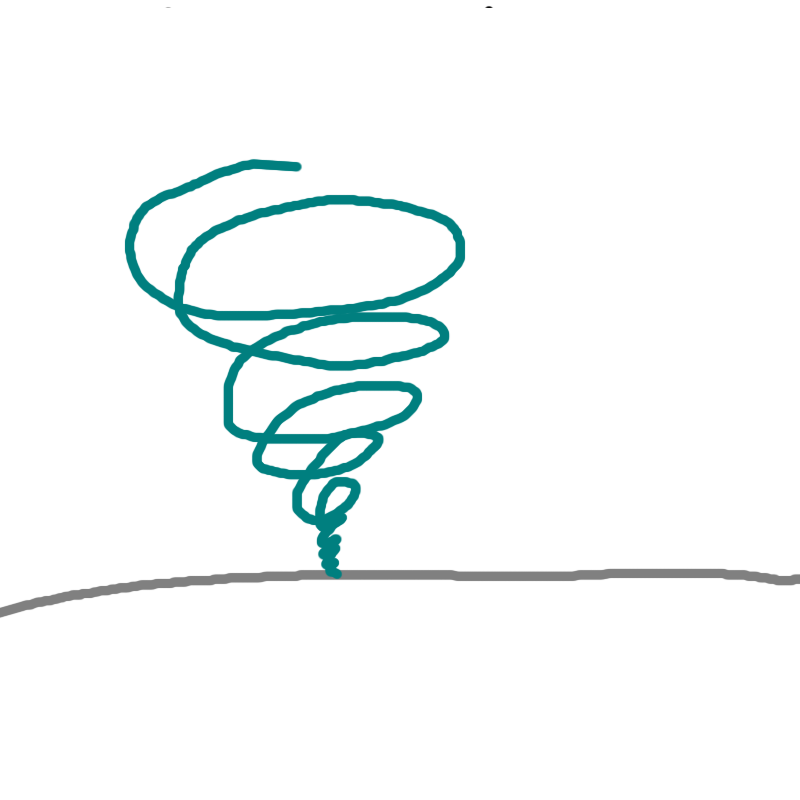
\includegraphics[height=0.2 \textheight]{Imagenes/tornado}
				\caption{Tornado.}
				\label{fig:tornado}
			\end{figure}

%============================================================
\section{Nombre: Ventisca.} \label{ventisca}
\subsection{Descripción}
El enemigo dispara una secuencia de cristales de hielo de manera repetida durante un periodo de tiempo. El disparo de estos cristales se dará en la dirección hacia la que este mirando el enemigo. Cada cristal reduce la cantidad de vida del jugador al colisionar con él. Los cristales se destruirán al colisionar con otro objeto que no sea el jugador o después de un tiempo si no han colisionado con ningún objeto.
\subsection{Portador}
Mictlecayotl (ver apartado \ref{per:mictlecayotl}).
\subsection{Esquema}
			Ver figura \ref{fig:ventisca}.
			\begin{figure}
				\centering
				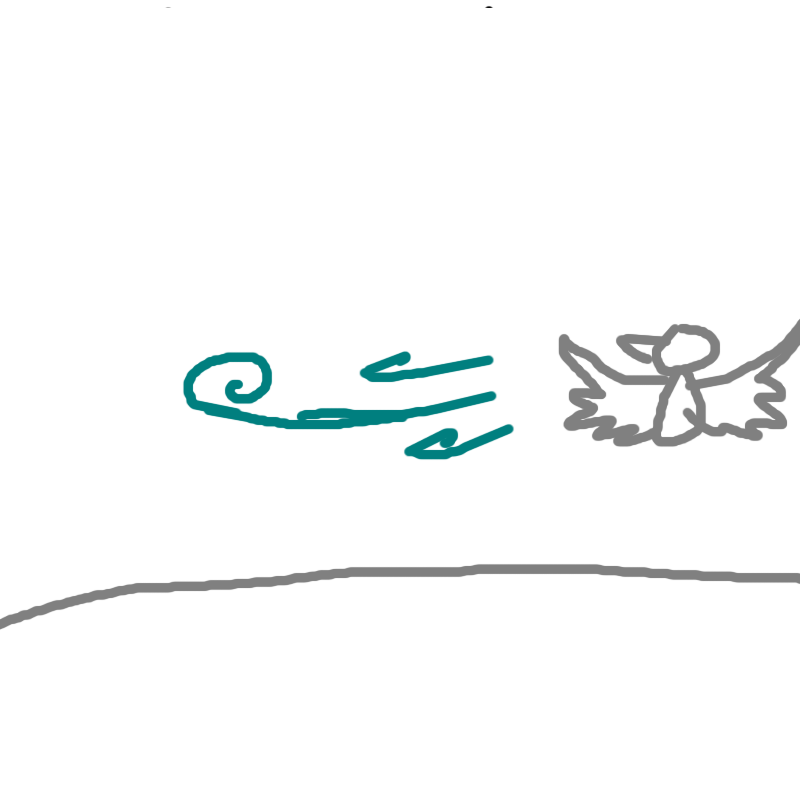
\includegraphics[height=0.2 \textheight]{Imagenes/ventisca}
				\caption{Ventisca.}
				\label{fig:ventisca}
			\end{figure}

%============================================================
\section{Nombre: Raíz del diablo.}\label{hab.RaizDia}
\subsection{Descripción}
Onda roja que produce confusión en el jugador por un periodo de tiempo determinado al hacer contacto con él. La onda incrementara su diámetro hasta alcanzar un diámetro máximo, una vez alcanzado ese diámetro máximo desaparecerá. Bajo el estado de confusión los controles de la GUI no responderán de manera efectiva intercambiando funcionalidad, es decir el botón de saltar moverá al personaje a la derecha, el botón de disparo será para saltar, el botón de mover hacia la izquierda será para disparar y el botón de mover hacia derecha moverá al personaje a la izquierda. 
\subsection{Portador}
Tlazoltéotl (ver apartado \ref{per:tlazolteotl}).
\subsection{Esquema}
			Ver figura \ref{fig:raiz}.
			\begin{figure}
				\centering
				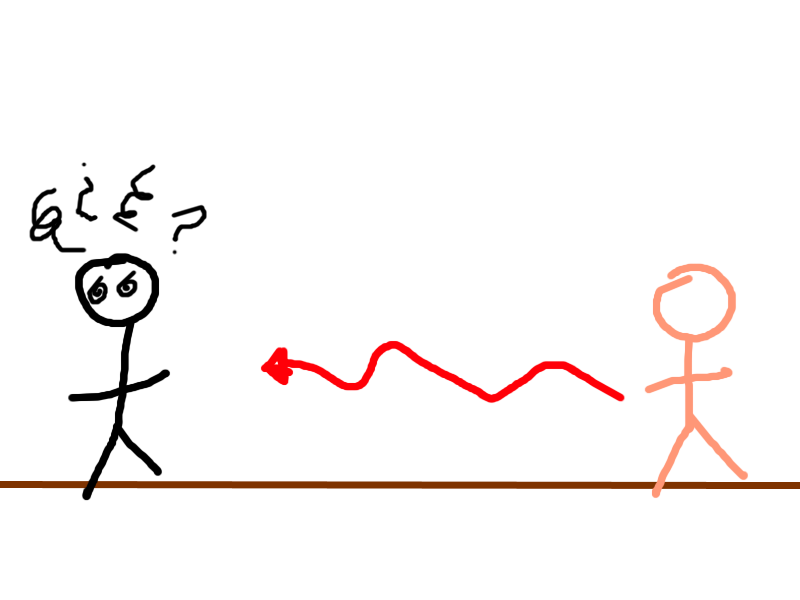
\includegraphics[height=0.2 \textheight]{Imagenes/raiz}
				\caption{Raíz del diablo.}
				\label{fig:raiz}
			\end{figure}

%============================================================
\section{Nombre: Energía corrupta.} \label{hab.CorrupEner}
\subsection{Descripción}
El enemigo dispará esferas de tonalli corrupto. las esferas seguirán al jugador durante un periodo de tiempo determinado. Cada esfera reduce la barra de vida del jugador de manera individual al hacer colisión con el jugador. Las esferas se destruyen al hacer contacto con el jugador, al colisionar con cualquier otro objeto o después de un tiempo si no han colisionado con ningún objeto o con el jugador. Las eferas solo afectaran al jugador al hacer contacto con el, si colisionan con otro objeto no afectarán a ese objeto. 
\subsection{Portador}
Tlazoltéotl (ver apartado \ref{per:tlazolteotl}).
\subsection{Esquema}
			Ver figura \ref{fig:energiaC}.
			\begin{figure}
				\centering
				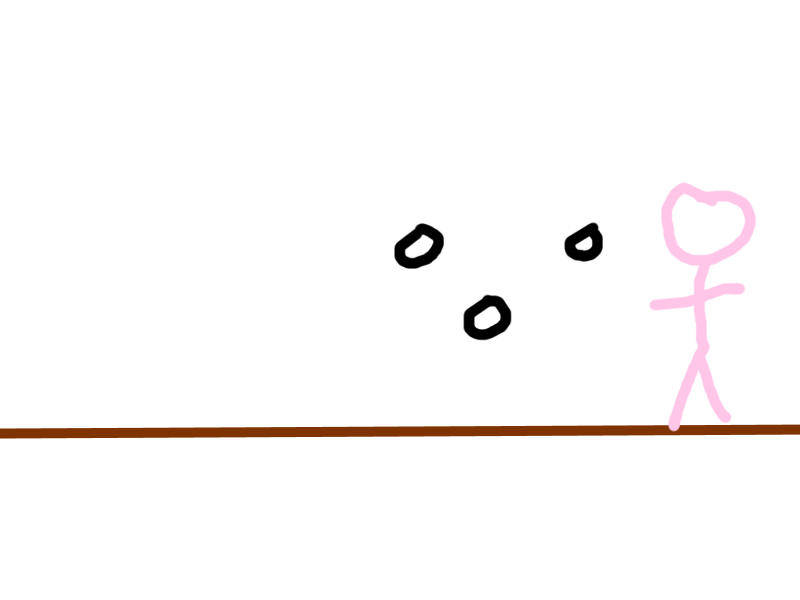
\includegraphics[height=0.2 \textheight]{Imagenes/energiaC}
				\caption{Energía corrupta.}
				\label{fig:energiaC}
			\end{figure}	

%============================================================
\section{Nombre: Circulo protector.} \label{hab.CirPro}
\subsection{Descripción}
El enemigo se rodea a sí mismo con un circulo de tonalli corrupto. El circulo reducirá la cantidad de vida del jugador al hacer contacto con éste. El fuego no afectara a otros objetos que no sean el jugador. Mientras esta habilidad se encuentre activa, el enemigo no recibirá daño por parte del jugador. La única manera de desactivar esta habilidad es que el jugador destruya el circulo protector disparando tonalli de manera constante. 
\subsection{Portador}
Tlazoltéotl (ver apartado \ref{per:tlazolteotl}).
\subsection{Esquema}
			Ver figura \ref{fig:circuloP}.
			\begin{figure}
				\centering
				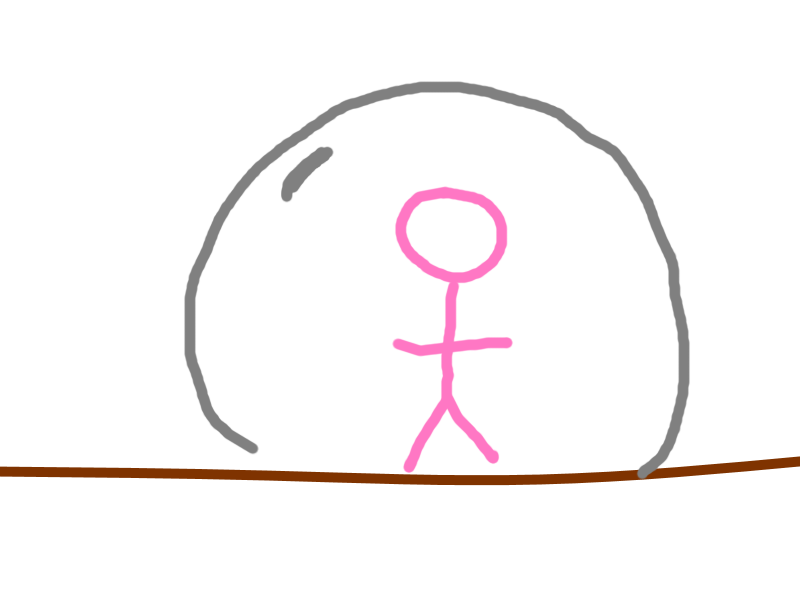
\includegraphics[height=0.2 \textheight]{Imagenes/circuloP}
				\caption{Círculo protector.}
				\label{fig:circuloP}
			\end{figure}

%============================================================
\section{Nombre: LLuvia de lava.} \label{hab.LLuviaLava}
\subsection{Descripción}
Caen bolas de lava del cielo en posiciones aleatorias. Las bolas de lava se destruyen al colisionar con el suelo, con una plataforma o con el jugador. Cuando una de las bolas de lava colisiona con el jugador disminuye la cantidad de vida del jugador, es decir cada bola de lava genera daño de manera individual. Las bolas de lava no pueden destruir las plataformas o el suelo al colisionar contra estas.
\subsection{Portador}
Itztlacoliuhqui (ver apartado \ref{per:itztlacoliuhqui}), Mictlantechtli (ver apartado \ref{per:mictlantechtli}).	
\subsection{Esquema}	
			Ver figura \ref{fig:lluviaL}.
			\begin{figure}
				\centering
				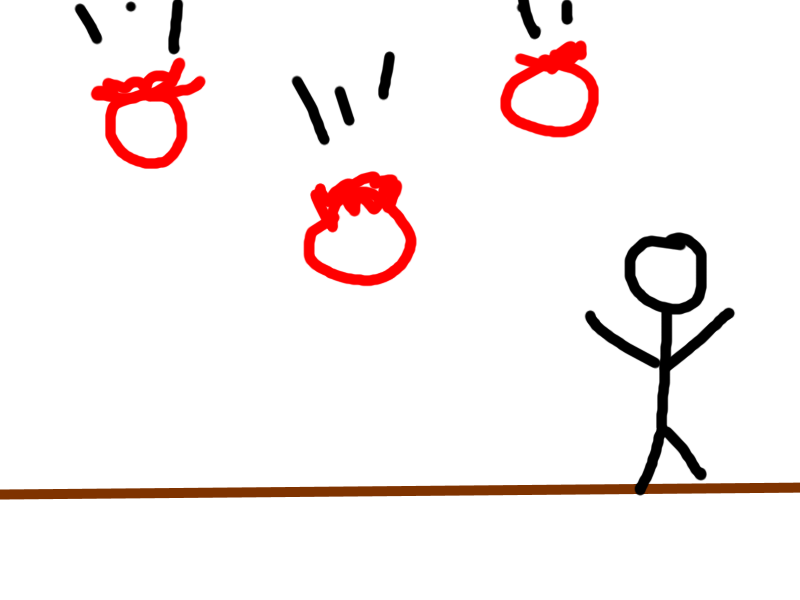
\includegraphics[height=0.2 \textheight]{Imagenes/lluviaL}
				\caption{Lluvia de lava.}
				\label{fig:lluviaL}
			\end{figure}

%============================================================
\section{Nombre: Manotazo.} \label{hab.Manotazo}
\subsection{Descripción}
El enemigo estrella su mano en el suelo, provocando una onda de piedras en el suelo. El avance de las piedras se hará de manera horizontal. Las piedras infringirán disminuirán la barra de vida del jugador al hacer contacto con el. Después de un tiempo las piedras desaparecerán.
\subsection{Portador}
Itztlacoliuhqui (ver apartado \ref{per:itztlacoliuhqui}).
\subsection{Esquema}
			Ver figura \ref{fig:manotazo}.
			\begin{figure}
				\centering
				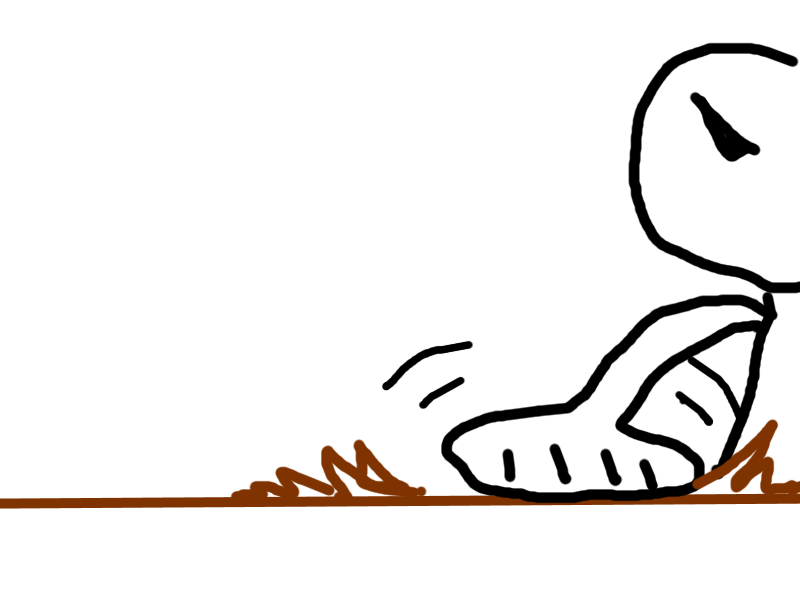
\includegraphics[height=0.2 \textheight]{Imagenes/manotazo}
				\caption{Manotazo.}
				\label{fig:manotazo}
			\end{figure}
Itztlacoliuhqui.

%============================================================
\section{Nombre: Lluvia de flechas.} \label{hab.LluviaFle}
\subsection{Descripción}
Caen flechas del cielo en posiciones aleatorias. Las flechas se destruyen al colisionar con el suelo, con una plataforma o con el jugador. Cuando una de las flechas colisiona con el jugador disminuye la cantidad de vida del jugador, es decir cada flecha genera daño de manera individual. Las flechas no pueden destruir las plataformas o el suelo al colisionar contra estas.
\subsection{Portador}
Itztlacoliuhqui (ver apartado \ref{per:itztlacoliuhqui}).
\subsection{Esquema}
			Ver figura \ref{fig:lluviaF}.

%============================================================
\section{Nombre: Todos los hombres del rey.}\label{hab.TodoRey}
\subsection{Descripción}
El portador de esta habilidad se posiciona en el centro de la vista de la cámara e invoca un portal del que salen cinco enemigos de estatus enemigo normal. El portador de la habilidad desaparece del campo de batalla y reaparece una vez que el jugador haya derrotado a todos los enemigos que se invocaron.  
\subsection{Portador}
Mictlantechtli (ver apartado \ref{per:mictlantechtli}).	
\subsection{Esquema}
			Ver figura \ref{fig:rey}.
			\begin{figure}
				\centering
				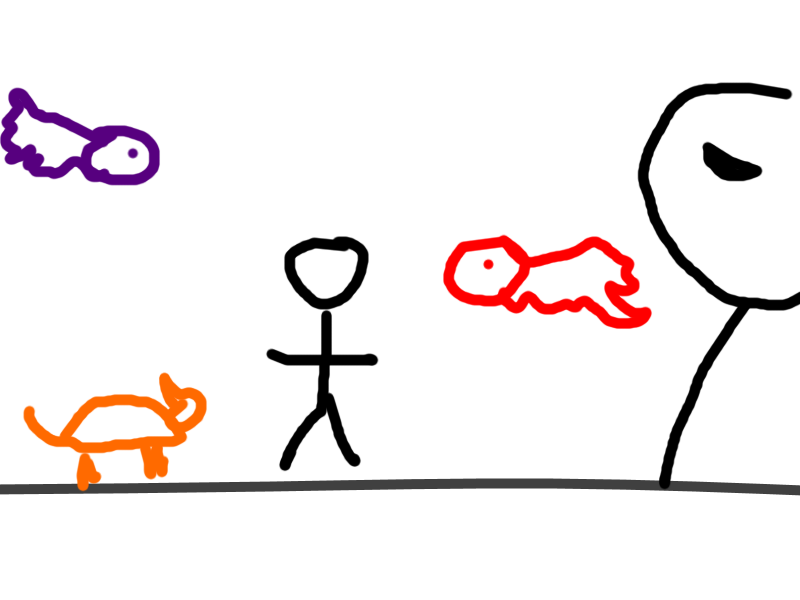
\includegraphics[height=0.2 \textheight]{Imagenes/rey}
				\caption{Todos los hombres del rey.}
				\label{fig:rey}
			\end{figure}
%============================================================
\section{Nombre: Fuego mortífero.} \label{hab.FuegoMor}
\subsection{Descripción}
El enemigo dispará esferas de fuego verde. Las esferas seguirán al jugador durante un periodo de tiempo determinado. Cada esfera reduce la barra de vida del jugador de manera individual al hacer colisión con el jugador. Las esferas se destruyen al hacer contacto con el jugador, al colisionar con cualquier otro objeto o después de un tiempo si no han colisionado con ningún objeto o con el jugador. Las eferas solo afectaran al jugador al hacer contacto con el, si colisionan con otro objeto no afectarán a ese objeto. 
\subsection{Portador}
Mictlantechtli (ver apartado \ref{per:mictlantechtli}).	
\subsection{Esquema}	
			Ver figura \ref{fig:fuegoM}.
			\begin{figure}
				\centering
				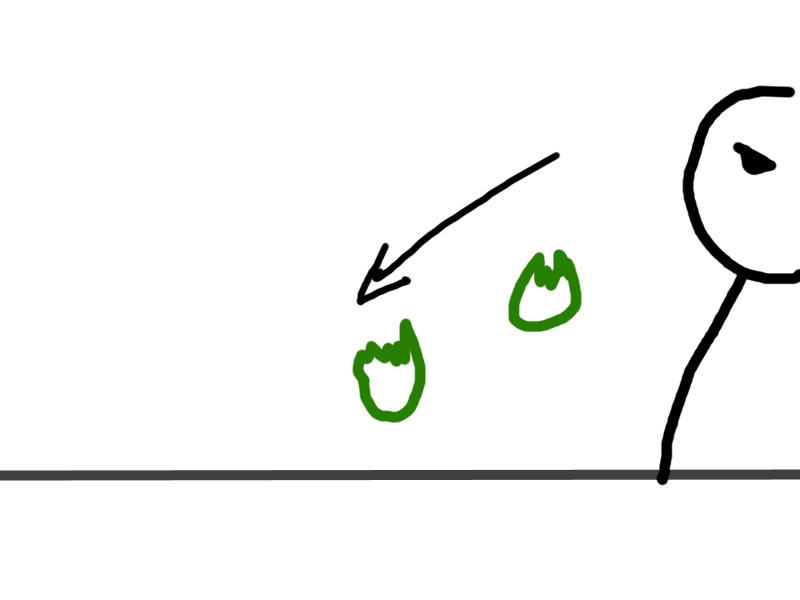
\includegraphics[height=0.2 \textheight]{Imagenes/fuegoM}
				\caption{fuegoM.}
				\label{fig:fuegoM}
			\end{figure}
%============================================================
\section{Nombre: Penitencia.}\label{hab.Penitencia}
\subsection{Descripción}
El enemigo hace que salgan huesos del suelo. El avance de las piedras se hará de manera horizontal. Las piedras infringirán disminuirán la barra de vida del jugador al hacer contacto con el. Después de un tiempo las piedras desaparecerán.
\subsection{Portador}
Mictlantechtli (ver apartado \ref{per:mictlantechtli}).	
\subsection{Esquema}
			Ver figura \ref{fig:penitencia}.
			\begin{figure}
				\centering
				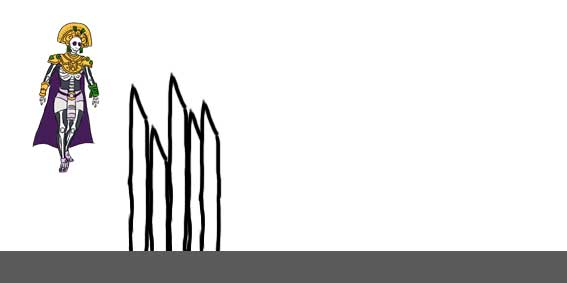
\includegraphics[height=0.2 \textheight]{Imagenes/penitencia}
				\caption{Penitencia.}
				\label{fig:penitencia}
			\end{figure}

%============================================================
\section{Nombre: Lluvia de huesos.}\label{hab.LluHuesos}
\subsection{Descripción}
Caen huesos del cielo en posiciones aleatorias. Los huesos se destruyen al colisionar con el suelo, con una plataforma o con el jugador. Cuando una de los huesos colisiona con el jugador disminuye la cantidad de vida del jugador, es decir cada hueso genera daño de manera individual. Los huesos no pueden destruir las plataformas o el suelo al colisionar contra estas.
\subsection{Portador}
Mictlantechtli (ver apartado \ref{per:mictlantechtli}).	
\subsection{Esquema}
			Ver figura \ref{fig:penitencia}.
			\begin{figure}
				\centering
				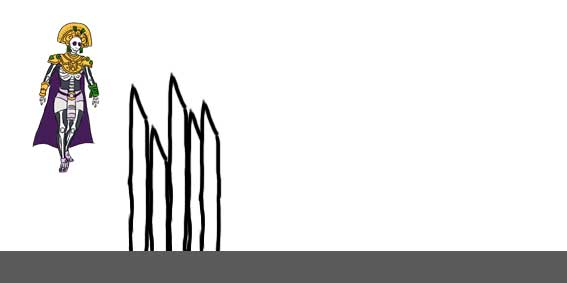
\includegraphics[height=0.2 \textheight]{Imagenes/penitencia}
				\caption{Penitencia.}
				\label{fig:penitencia}
			\end{figure}
			
%============================================================
\section{Nombre: Estocada mortífera.}\label{hab.estMor}
\subsection{Descripción}
Se invoca un solo hueso gigante con forma de cuchilla que recorre el campo de manera horizontal a la altura del suelo con gran velocidad. El hueso disminuirá la cantidad de vida del jugador al hacer contacto con éste. El hueso desaparecerá al finalizar su recorrido.
\subsection{Portador}
Mictlantechtli (ver apartado \ref{per:mictlantechtli}).	
\subsection{Esquema}
			Ver figura \ref{fig:penitencia}.
			\begin{figure}
				\centering
				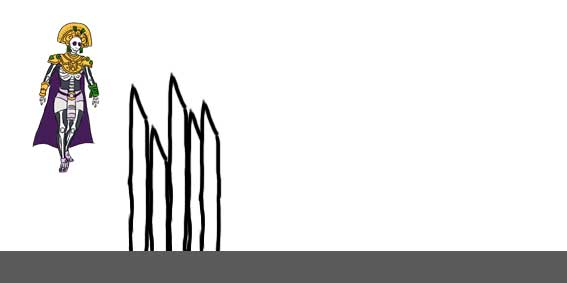
\includegraphics[height=0.2 \textheight]{Imagenes/penitencia}
				\caption{Penitencia.}
				\label{fig:penitencia}
			\end{figure}			
			